\documentclass[11pt,a4paper]{article}

\usepackage[margin=1in, paperwidth=8.3in, paperheight=11.7in]{geometry}
\usepackage{amsfonts}
\usepackage{amsmath}
\usepackage{enumerate}
\usepackage{enumitem}
\usepackage{fancyhdr}
\usepackage{graphicx}

\begin{document}

\pagestyle{fancy}
\setlength\parindent{0pt}
\allowdisplaybreaks

\renewcommand{\headrulewidth}{0pt}

% Cover page title
\title{Multi-Variable Calculus - Notes}
\author{Dom Hutchinson}
\date{\today}
\maketitle

% Header
\fancyhead[L]{Dom Hutchinson}
\fancyhead[C]{Multi-Variable Calculus - Notes}
\fancyhead[R]{\today}

% Counters
\newcounter{definition}[section]
\newcounter{notation}[section]
\newcounter{proposition}[section]
\newcounter{remark}[section]
\newcounter{theorem}[section]

% commands
\newcommand{\definition}[1]{\stepcounter{definition} \textbf{Definition \arabic{section}.\arabic{definition}\ - }\textit{#1}\\}
\newcommand{\dotprod}[0]{\boldsymbol{\cdot}}
\newcommand{\cosech}[0]{\mathrm{cosech}\ }
\newcommand{\cosec}[0]{\mathrm{cosec}\ }
\newcommand{\sech}[0]{\mathrm{sech}\ }
\newcommand{\nats}[0]{\mathbb{N}}
\newcommand{\real}[0]{\mathbb{R}}
\newcommand{\notation}[1]{\stepcounter{notation} \textbf{Notation \arabic{section}.\arabic{notation}\ - }\textit{#1}\\}
\newcommand{\proposition}[1]{\stepcounter{proposition} \textbf{Proposition \arabic{section}.\arabic{proposition}\ - }\textit{#1}\\}
\newcommand{\remark}[1]{\stepcounter{remark} \textbf{Remark \arabic{section}.\arabic{remark}\ - }\textit{#1}\\}
\newcommand{\theorem}[1]{\stepcounter{theorem} \textbf{Theorem \arabic{section}.\arabic{theorem}\ - }\textit{#1}\\}

\tableofcontents

% Start of content
\newpage

\section{Review of Differential Calculus with Multi-Variable Functions}

\subsection{General Maps, $\real^m \to \real^n$}

\definition{Scalar Map}
A \textit{scalar map} maps a real-valued vector to a single real value.\\
They can be represented by the signature $f : \real^n \to \real, n \in \nats$.\\

\definition{Vector Map}
A \textit{vector map} maps a real-valued vector to another real-valued vector.\\
They can be represented by the signature $\textbf{F} : \real^m \to \real^n,\ m,n \in \real$.\\
\textit{Vector map}s can be considered as a collection of linear maps, so can be considered as $$\textbf{F}(\textbf{x}) = \begin{pmatrix} F_1(\textbf{x}) \\ \vdots \\ F_n(\textbf{x})\end{pmatrix} \quad F_i : \real^m \to \real, i=\{1, \dots, n\}, \textbf{x} \in \real^m$$.

\definition{Linear Map}
A general map, $\textbf{F} : \real^m \to \real^n$, is \textit{linear} if
$$\forall\ \textbf{x}, \textbf{y} \in \real^m\ \&\ \lambda,\ \mu \in \real,\  \textbf{F}(\lambda\textbf{x}+\mu\textbf{y})=\lambda\textbf{F}(\textbf{x})+\mu\textbf{F}(\textbf{y})$$

\proposition{Linear Maps as Matrices}
$\forall$ \textit{linear maps}, $\textbf{F} : \real^m \to \real^n\ \exists\ A \in M_{n,m}(\real)\ st\ \textbf{F}(\textbf{x})=A\textbf{x}$.\\

\subsection{Derivative of a Map}

\definition{Derivative}
The \textit{derivative} of a general map, $\textbf{F} : \real^m \to \real^n$, is an $n\times m$ matrix, $\textbf{F}'$ st $\{\textbf{F}'(\textbf{x})\}_{ij}=\frac{\partial F_i}{\partial x_j}$.\\

\definition{Derivative of Single Variable Linear Maps}
The \textit{derivative} of a single variable linear map, $f : \real \to \real$, is the map, $f' : \real \to \real$, st the line formed by $$y=f(x_0)+(x-x_0)f'(x_0)$$ is the tangent to $f$ at $x-x_0$.\\

\definition{Derivative of a Single Variable Map}
The \textit{derivative}, $f'$, of a single variable map, $f :\real\to\real$, can be defined as a limit
$$f'(x)=\lim_{h\to0}\frac{f(x+h)-f(x)}{h}$$

\definition{Derivative of Multi-Variable Maps}
The \textit{derivative} of a multi-variable map, $\textbf{F} : \real^m \to \real^n$, is a matrix, $\textbf{F}' \in M_{n,m}$, st $\textbf{F}(\textbf{x}_0)+\textbf{F}'(\textbf{x}_0)(\textbf{x} - \textbf{x}_0 )$ is a tangent plane at $\textbf{x}=\textbf{x}_0$ to the \textit{hyper surface} of $\textbf{F}(\textbf{x})$.\\

\newpage
\proposition{Derivative of a Linear Map}
If a map $\textbf{F} : \real^m \to \real^n$ is linear st $\textbf{F}(\textbf{x}) = A\textbf{x},\ A \in M_{n,m}$.\\
Then $\textbf{F}'(\textbf{x}) = A$.\\
\textbf{Proof}
\[\begin{array}{rrcl}
  \mathrm{We\ know} &\textbf{F}_i&=&\sum_{k=1}^m A_{ik}x_k\\
  \implies& \frac{\partial F_i}{\partial x_j} &=& \{\textbf{F}'\}_{ij}\\
  &&=& \sum_{k=1}^m A_{ik} \frac{\partial x_k}{\partial x_j}\\
  &&=& \sum_{k=1}^m A_{ik} \delta_{kj}\\
  &&=& A_{ij}
\end{array}\]

\definition{Jacobian Matrix}
The matrix, $A$, produced by the derivative of a vector map $\textbf{F}:\real^m\to\real^n$, with elements $A_{ij}=\frac{\partial F_i}{\partial x_j}$, is called the \textit{Jacobian Matrix}.\\

\subsection{The Gradient of a Function}

\definition{Gradient of a Scalar Function}
The \textit{gradient} of a scalar function, $f : \real^m \to \real$, is defined as
$$\nabla f = \begin{pmatrix} \frac{\partial f}{\partial x_1} \\ \vdots \\ \frac{\partial f}{\partial x_m}\end{pmatrix}$$

\remark{Jacobian Matrix as Vector of Gradients}
Each row of a \textit{Jacobian Matrix} can be considered as the \textit{gradient} of that component of the  map, as each component is scalar.
$$\textbf{F}' = \begin{pmatrix} \nabla F_1^T \\ \vdots \\ \nabla F_n^T\end{pmatrix}$$

\subsection{Directional Derivative}

\definition{Directional Derivative}
The \textit{directional derivative} of a map gives the rate of change in a given direction.\\
For a map, $\textbf{F} : \real^m \to \real^n$, at a given point, $\textbf{x}_0 \in \real^m$, in the given direction, $\textbf{\^v} \in \real^m$, the \textit{directional derivative} is a vector in $\real^n$ given by the formula
$$D_{\textbf{\^v}}\textbf{F}(\textbf{x}_0) = \begin{pmatrix} \frac{d}{dt} F_1 (\textbf{x}_0 + t \textbf{\^v})|_{t=0} \\ \vdots \\ \frac{d}{dt} F_n (\textbf{x}_0 + t \textbf{\^v})|_{t=0} \end{pmatrix}$$
This can be simplified to
$$D_\textbf{\^v}\textbf{F}(\textbf{x}_0) = \textbf{F}'(\textbf{x}_0)\textbf{\^v}$$
\textbf{Proof}
\[\begin{array}{rcl}
D_{\textbf{\^v}} \textbf{F}(\textbf{x}_0) &=& \frac{d}{dt} \textbf{F} (\textbf{x}_0 + t \textbf{\^v})\big\vert_{t=0}\\
&=& \lim_{h\to 0} \frac{\textbf{F}(\textbf{x}_0 + (t+h)\textbf{\^v}) - \textbf{F}(\textbf{x}_0 + t\textbf{\^v})}{h}\big\vert_{t=0}\\
&=& \lim_{h\to 0} \frac{\textbf{F}(\textbf{x}_0 + h\textbf{\^v}) - \textbf{F}(\textbf{x}_0)}{h}\\
&=& \lim_{h\to 0} \frac{\textbf{F}(\textbf{x}_0) + \textbf{F}'(\textbf{x}_0)(\textbf{x}_0 + h\textbf{\^v} - \textbf{x}_0) - \textbf{F}(\textbf{x}_0)}{h}\\
&=& \lim_{h\to 0} \textbf{F}'(\textbf{x}_0)\textbf{\^v}\\
&=& \textbf{F}'(\textbf{x}_0)\textbf{\^v}
\end{array}\]

\remark{Directional Derivative of a Scalar Map}
For a scalar map, $f : \real^m \to \real$,  the \textit{directional derivative} is simplified to
$$D_\textbf{\^v}f(\textbf{x}_0) = \nabla f \dotprod \textbf{\^v} \in \real$$

\subsection{Operations on Maps \& their Derivatives}

\theorem{Derivative of Map Sums}
Let $\textbf{F}, \textbf{G}, \textbf{H} : \real^m \to \real^n$ st $\textbf{H} = \textbf{F} + \textbf{G}$.\\
Then $\textbf{H}' = \textbf{F}' + \textbf{G}'$.\\
\textbf{Proof}
\[\begin{array}{rcl}
  \textbf{H}' &=& \frac{\partial H_i}{\partial x_j}\\
  &=& \frac{\partial}{\partial x_j} (F_i + G_i)\\
  &=& \frac{\partial F_i}{\partial x_j} + \frac{\partial G_i}{\partial x_j}\\
  &=& \textbf{F}' + \textbf{G}'
\end{array}\]

\theorem{Derivative of Scalar \& Vector Map Compositions}
Let $\textbf{F}, \textbf{H} : \real^m \to \real^n$ \& $f:\real^m \to \real$ st $\textbf{H}(\textbf{x})=f(\textbf{x})\textbf{F}(\textbf{x})$.\\
Then
\[\begin{array}{rcl}
\{\textbf{H}'(\textbf{x})\}_{ij} &=& \frac{\partial}{\partial x_j} \left[f(\textbf{x})F_i((\textbf{x}))\right]\\
&=& \frac{\partial f}{\partial x_j}(\textbf{x}) F_i(\textbf{x}) + f(\textbf{x}) \frac{\partial F_i}{\partial x_j}(\textbf{x})
\end{array}\]

\theorem{Chain Rule for Multi-Variable Functions}
Let $\textbf{F} : \real^m \to \real^n, \textbf{G} : \real^n \to \real^p\ \&\  {H} : \real^m \to \real^p$.\\
Define $\textbf{H}=\textbf{G} \dotprod \textbf{F}$. Then
$$\textbf{H}'(\textbf{x})=(\textbf{G}' \dotprod \textbf{F})(\textbf{x})\textbf{F}'(\textbf{x})$$
\textbf{Proof}\\
Note that $H_i = G_i\begin{pmatrix} F_1(x_1, \dots, x_m) \\ \vdots \\ F_n(x_1, \dots, x_m)\end{pmatrix}$.\\
\[\begin{array}{rrcl}
\implies& {\textbf{H}'}_{ij}&=&\frac{\partial H_i}{\partial x_j}\\
&&=&\frac{\partial G_i}{\partial x_1}\frac{\partial F_1}{\partial x_j} + \dots + \frac{\partial G_i}{\partial x_n}\frac{\partial F_n}{\partial x_j}\\
&&=&\sum_{k=1}^n\frac{\partial G_i}{\partial x_k} \dotprod \frac{\partial F_k}{\partial x_j}
\end{array}\]

\subsection{Inverse Maps}

\definition{Inverse Map}
Let $\textbf{F}, \textbf{G} : \real^n \to \real^n$.\\
$\textbf{G}$ is the \textit{inverse map} of $\textbf{F}$ if $(\textbf{G} \dotprod \textbf{F})(\textbf{x}) = \textbf{x}$.\\
Then, $\textbf{G}$ can be written as $\textbf{G} = \textbf{F}^{-1}$.\\

\remark{Inverse Derivative}
Since $(\textbf{F}^{-1}\dotprod\textbf{F})(\textbf{x}) = \textbf{x} = I\textbf{x}$, where $I$ is the identity matrix.\\
By differentiating we find $\textbf{F}^{-1} \dotprod \textbf{F} = (\textbf{F}^{-1})' (\textbf{F}(\textbf{x}))\ \textbf{F}'(\textbf{x}) = I$.\\
Thus $(\textbf{F}^{-1})'(\textbf{F}(\textbf{x})) = (\textbf{F}'(\textbf{x}))^{-1}$.
\begin{center}
\textit{The derivative of the inverse = Inverse of the derivative}.\\
$g'(f)=(f'(g))^{-1}$
\end{center}

\remark{Solving Inverse Derivatives}
Let $\textbf{F}:\real^m\to\real^n$ be a general map and $\textbf{x}\in\real^m$. Then
$$(\textbf{F}^{-1}(\textbf{x}))'=\frac{1}{\textbf{F}'(\textbf{F}^{-1}(\textbf{x}))}$$

\remark{When is a Matrix Invertible?}
A matrix $A$ is \textit{invertible} if $det(A)\neq0$.

\subsection{Solving Equations}

\definition{Jacobian Determinant}
Let $\textbf{F} : \real^n\to\real^n$ be a general map.\\
The \textit{Jacobian Determinant} is the determinant of the Jacobian Matrix of $\textbf{F}$.
$$J_{\textbf{F}}(\textbf{x}_0) := \frac{\partial(F_1, \dots, F_n)}{\partial(x_1, \dots, x_n)}\bigg\vert_{\textbf{x}=\textbf{x}_0}$$
\textbf{Proof} (\textit{Informal})\\
For $\textbf{x}\in\real^m$ close to $\textbf{x}_0$ we can use $\textbf{F}(\textbf{x}_0)+\textbf{F}'(\textbf{x}_0)(\textbf{x}-\textbf{x}_0)$ to approximate $\textbf{F}(\textbf{x})$.\\
So\[\begin{array}{rrcl}
&y&=&\textbf{F}(\textbf{x})\\
&&\approx& \textbf{F}(\textbf{x}_0)+\textbf{F}'(\textbf{x}_0)(\textbf{x}-\textbf{x}_0)\\

\implies&\textbf{x}&\approx&\textbf{x}_0+[\textbf{F}'(\textbf{x}_0)]^{-1}(\textbf{y}-\textbf{y}_0)\\
\end{array}\]
Since $\textbf{y}_0 = \textbf{F}(\textbf{x}_0)$ but relies on the existence of the inverse of the Jacobian.\\

\theorem{Inverse Function Theorem}
Let $\textbf{F} : \real^n \to \real^n\ \&\ \textbf{x}_0,\textbf{y}_0 \in \real^n$ st $\textbf{y}_0=\textbf{F}(\textbf{x}_0)$.\\
The \textit{Inverse Function Theorem} states
\begin{center}If $J_\textbf{F}(\textbf{x}_0))\neq0$ then $\textbf{y}=\textbf{F}(\textbf{x})$ can be solved uniquely as $\textbf{x}=\textbf{F}^{-1}(\textbf{y})$ for $\textbf{y}$ in the neighbourhood of $\textbf{y}_0$.\end{center}

\remark{Inverse Function Theorem \& Lack of Inverse}
The \textit{Inverse Function Theorem} does not say anything about the case where the inverse does not exists.\\

\definition{Implicit Function}
An \textit{implicit function} is a function in which one variable cannot be explicitly expressed in terms of another.\\
\textit{Example} - $x^2+y^2=1$.\\

\theorem{Implicit Function Theorem}
Consider $\textbf{x} \in\real^m,\ \textbf{y}\in\real^n\ \&\ \textbf{F} : \real^{m+n} \to \real^n$ where $\textbf{F}$ a system of non-linear equations.\\
Suppose $\textbf{F}(\textbf{x},\textbf{y})=\textbf{0}$ is satisfied by $(\textbf{x}_0, \textbf{y}_0)$.\\
The \textit{Implicit Function Theorem} states
\begin{center}If $J_{\textbf{F}}(\textbf{x}_0,\textbf{y}_0)\neq0$ we  can express $\textbf{F}(\textbf{x},\textbf{y})=\textbf{0}$ in the form $\textbf{y}=\textbf{y}(\textbf{x})$ for $\textbf{y} : \real^m \to \real^n$ in the neighbourhood of $\textbf{y}_0$.
\end{center}

\textbf{Proof} \textit{(Informal)}\\
The $i^{th}$ component of $\textbf{F}(\textbf{x}_0, \textbf{y}_0) = \textbf{0}$ is $F_i(x_1, \dots, x_n, y_1, \dots, y_n) = 0$\\
but $y_i=y_i(x_1, \dots, x_n) \forall\ i \in [1, n]$\\
So by taking $\frac{\partial F_i}{\partial x_j}$ and, using the chain rule, we get
$$\frac{\partial F_i}{\partial x_j} + \frac{\partial F_i}{\partial y_1}.\frac{\partial y_1}{\partial x_j} + \dots +\frac{\partial F_i}{\partial y_n}.\frac{\partial y_n}{\partial x_j}=0$$
This can be expressed as
\[\begin{array}{rl}
&\begin{pmatrix}
\frac{\partial F_1}{\partial x_1} & \dots & \frac{\partial F_1}{\partial x_m}\\
\vdots & \ddots & \vdots\\
\frac{\partial F_n}{\partial x_1} & \dots & \frac{\partial F_n}{\partial x_m}
\end{pmatrix} +\begin{pmatrix}
\frac{\partial F_1}{\partial y_1} & \dots & \frac{\partial F_1}{\partial y_n}\\
\vdots & \ddots & \vdots\\
\frac{\partial F_n}{\partial y_1} & \dots & \frac{\partial F_n}{\partial y_n}
\end{pmatrix} \begin{pmatrix}
\frac{\partial y_1}{\partial x_1} & \dots & \frac{\partial y_1}{\partial x_m}\\
\vdots & \ddots & \vdots\\
\frac{\partial y_n}{\partial x_1} & \dots & \frac{\partial y_n}{\partial x_m}
\end{pmatrix} = 0 \\
\implies& \begin{pmatrix}
\frac{\partial y_1}{\partial x_1} & \dots & \frac{\partial y_1}{\partial x_m}\\
\vdots & \ddots & \vdots\\
\frac{\partial y_n}{\partial x_1} & \dots & \frac{\partial y_n}{\partial x_m}
\end{pmatrix} = - \begin{pmatrix}
\frac{\partial F_1}{\partial y_1} & \dots & \frac{\partial F_1}{\partial y_n}\\
\vdots & \ddots & \vdots\\
\frac{\partial F_n}{\partial y_1} & \dots & \frac{\partial F_n}{\partial y_n}
\end{pmatrix}^{-1} \begin{pmatrix}
\frac{\partial F_1}{\partial x_1} & \dots & \frac{\partial F_1}{\partial x_m}\\
\vdots & \ddots & \vdots\\
\frac{\partial F_n}{\partial x_1} & \dots & \frac{\partial F_n}{\partial x_m}
\end{pmatrix}
\end{array}\]
By \textbf{Definition 1.6} we have that, for $\textbf{x}$ near $\textbf{x}_0$,
\[\begin{array}{rcl}
\textbf{y} &\approx& \textbf{y}(\textbf{x}_0)+\textbf{y}'(\textbf{x}_0)(\textbf{x}-\textbf{x}_0)\\
&=&\textbf{y}_0+\textbf{y}'(\textbf{x}_0)(\textbf{x}-\textbf{x}_0)
\end{array}\]
So $\textbf{y}$ is near $\textbf{y}_0$ \underline{provided} $\textbf{y}'(\textbf{x}_0)$ exists. (\textit{i.e.} $J_{\textbf{F}}(\textbf{x}_0, \textbf{y}_0)\neq0$).\\

\remark{Linear Maps \& Implicit Function Theorem}
If $\textbf{F} : \real^{m+n} \to \real^n$ is linear in $\textbf{y}$ then $\textbf{F}(\textbf{x},\textbf{y})=\textbf{0}$ can be written in the form
$$\textbf{y} = \textbf{G}(\textbf{x})$$
Thus it can use the \textit{inverse function theorem}.

\subsection{Higher-Order Derivatives}

\stepcounter{remark} \textbf{Remark \arabic{section}.\arabic{remark}\ - }\textit{Second Order Derivatives}
$$\frac{\partial^2 F_i}{\partial x_j \partial x_k} = \frac{\partial^2 F_i}{\partial x_k \partial x_j}$$

\theorem{Taylor's Theorem for Single Variable Scalar Functions}
For scalar functions $f : \real \to \real$ \textit{Taylor's Theorem} states
\[\begin{array}{rcl}
f(x)&=&f(x_0)\\
&+&(x-x_0)f'(x_0)\\
&+&\frac{1}{2!}(x-x_0)^2f''(x_0)\\
&\vdots&\\
&+&\frac{1}{n!}(x-x_0)^nf^{(n)}(x_0)
\end{array}\]

\theorem{Taylor's Theorem for Double Variable Scalar Functions}
For scalar functions $f : \real^2 \to \real$ \textit{Taylor's the}
\[\begin{array}{rcl}
f(x,y) &=& f(x_0, y_0)\\
&+&\begin{pmatrix}f_x(x_0, y_0) & f_y(x_0, y_0)\end{pmatrix}\begin{pmatrix}x-x_0 \\ y-y_0\end{pmatrix}\\
&+&\frac{1}{2!}\begin{pmatrix}x-x_0 & y-y_0\end{pmatrix}\begin{pmatrix}f_{xx}(x_0, y_0) & f_{xy}(x_0,y_0)\\f_{yx}(x_0,y_0) &f_{yy}(x_0, y_0)\end{pmatrix}\begin{pmatrix}x-x_0 \\ y-y_0\end{pmatrix}\\
&+&\mathrm{higher\ order\ terms}
\end{array}\]

\remark{Taylor's Theorem - Vector Functions}
For vector functions, $\textbf{F} : \real^n \to \real^m$, each component is a scalar function so by \textit{Taylor's Theorem}
$$F_i(\textbf{x}) = f_i(\textbf{x}_0)+(\nabla f_i)^T(\textbf{x}-\textbf{x}_0) + \mathrm{higher\ order\ terms},\ \textbf{x}\in\real^m$$
Consider the whole function we get
$$\textbf{F}(\textbf{x})=\textbf{F}(\textbf{x}_0)+\textbf{F}'(\textbf{x}_0)(\textbf{x}-\textbf{x}_0)+\mathrm{higher\ order\ terms}$$
If $\textbf{x} \approx \textbf{x}_0$ \& $|\textbf{x}-\textbf{x}_0|^2 < |\textbf{x}-\textbf{x}_0|$ then
$$\textbf{F}(\textbf{x}) \approx \textbf{F}(\textbf{x}_0)+\textbf{F}'(\textbf{x}_0)(\textbf{x}-\textbf{x}_0)$$
Since the higher order terms tend to size $|\textbf{x}-\textbf{x}_0|^2$.
\section{Differential Vector Calculus}

\subsection{Linear Algebra}

\theorem{Sampling Property}
Using the \textit{Einstein summation convention}
$$x_i=\delta_{ij}x_j$$

\stepcounter{remark} \textbf{Remark \arabic{section}.\arabic{remark}\ - }\textit{Cross Product is Anti-Commutative}
$$\textbf{u}\times\textbf{v}=-\textbf{v}\times\textbf{u}$$
\textbf{Proof}
\[\begin{array}{rcl}
\textbf{u}\times\textbf{v}&=&\begin{pmatrix}
u_2v_3-u_3v_2\\
u_3v_1-u_1v_3\\
u_1v_2-u_2v_1
\end{pmatrix}\\
\textbf{v}\times\textbf{u}&=&\begin{pmatrix}
u_3v_2-u_2v_3\\
u_1v_3-u_3v_1\\
u_2v_1-u_1v_2
\end{pmatrix}\\
&=&\begin{pmatrix}
-(u_2v_3-u_3v_2)\\
-(u_3v_1-u_1v_3)\\
-(u_1v_2-u_2v_1)
\end{pmatrix}\\
&=&-\begin{pmatrix}
u_2v_3-u_3v_2\\
u_3v_1-u_1v_3\\
u_1v_2-u_2v_1
\end{pmatrix}\\
&=&-\textbf{u}\times\textbf{v}
\end{array}\]

\stepcounter{remark} \textbf{Remark \arabic{section}.\arabic{remark}\ - }\textit{Values of Levi-Civita Tensor in $\real^3$}
\[\begin{array}{rcr}
\mathcal{E}_{123}=\mathcal{E}_{231}=\mathcal{E}_{312}&=&1\\
\mathcal{E}_{231}=\mathcal{E}_{132}=\mathcal{E}_{321}&=&-1\\
\mathrm{All\ other\ cases}&=&0
\end{array}\]

\proposition{Cross Product with Levi-Civita Tensor Notation}
By expanding the first component of the cross product we find
\[\begin{array}{rcl}[\textbf{u}\times\textbf{v}]_1&=&u_2v_3-u_3v_2\\
&=&0.u_1v_1+0.u_1v_2+0.u_1v_3\\
&+&0.u_2v_1+0.u_2v_2+1.u_2v_3\\
&+&0.u_3v_1-1.u_3v_2+0.u_3v_3\\
&=&\sum_{j=1}^3\sum_{k=1}^3 \mathcal{E}_{1jk}u_jv_k\\
&=&\mathcal{E}_{1jk}u_jv_k
\end{array}\]
By considering the second \& third components we find
$$[\textbf{u}\times\textbf{v}]_i=\mathcal{E}_{ijk}u_jv_k$$

\proposition{Double Levi-Civita Tensor Product}
The formula for the product of two \textit{Levi-Civita tensor}s with one shared variable is given by
$$\mathcal{E}_{ijk}\mathcal{E}_{ilm}=\delta_{jl}\delta_{km}-\delta_{jm}\delta_{kl}$$
This is found by considering all combinations.\\
There are $81$ combinations but it is easy to discount most the zero-valued ones quickly.\\

\remark{Proving a Vector identity}
When proving a vector identity it is best to do so by comparing components.\\
\textit{i.e.} Show the $i^{th}$ component of $LHS$ = $i^{th}$ component of $rHS$.\\

\stepcounter{theorem} \textbf{Theorem \arabic{section}.\arabic{theorem}\ - }\textit{Vector Triple Product}
$$\textbf{a}\times(\textbf{b}\times\textbf{c}) = (\textbf{a}\dotprod\textbf{c})\textbf{b}-(\textbf{a}\dotprod\textbf{b})\textbf{c}$$
\textbf{Proof}
\[\begin{array}{rcl}
[\textbf{a}\times(\textbf{b}\times\textbf{c})]_i &=& \mathcal{E}_{ijk} a_j[\textbf{b}\times\textbf{c}]_k\\
&=& \mathcal{E}_{ijk}a_j \mathcal{E}_{klm} b_i c_m\\
\mathrm{By\ cycling\ } \mathcal{E}_{ijk}&=& \mathcal{E}_{ijk} \mathcal{E}_{klm} a_j b_i c_m\\
&=&(\delta_{il}\delta_{jm}-\delta_{im}\delta_{jl})a_jb_lc_m\\
&=&(\delta_{il}b_i)(\delta_{jm}c_ma_j)-(\delta_{im}c_m)(\delta_{jl}b_la_j)\\
&=&b_ic_ja_j-c_ib_ja_j\\
&=&(\textbf{c}\dotprod\textbf{a})b_i-(\textbf{b}\dotprod\textbf{a})c_i\\
&=&[(\textbf{a}\dotprod\textbf{c})\textbf{b}-(\textbf{a}\dotprod\textbf{b})\textbf{c}]_i
\end{array}\]
This is true for $i=1,2,3$.\\
Since it holds for all components, the result holds.

\subsection{Scalar \& Vector Fields}

\definition{Scalar Field}
A \textit{scalar field} on $\real^3$ is a function $f : \real^3\to\real$.\\

\definition{Vector Field}
A \textit{vector field} on $\real^3$ is a map $\textbf{v} : \real^3\to\real^3$.
$$\textbf{v}(\textbf{r})=(v_1(\textbf{r}), v_2(\textbf{r}), v_3(\textbf{r}))$$
where $v_i(\textbf{r})$ are scalar fields for $i=1,2,3$.\\

\remark{Some Physical Applications of Scalar \& Vector Fields}
Scalar Applications
\begin{enumerate}[label=\roman*)]
  \item Temperature$, T(\textbf{q})$;
  \item Density, $\rho(\textbf{r})$;
  \item Electric Charge Density, $q(\textbf{r})$.
\end{enumerate}
Vector Applications
\begin{enumerate}[label=\roman*)]
  \item Velocity, $\textbf{v}(\textbf{r})$;
  \item Displacement, $\textbf{s}(\textbf{r})$.
\end{enumerate}
All of these quantities are governed by differential equations in space (and time) \& require integration to find.

\subsection{Gradient}

\definition{Gradient of Scalar Fields}
A \textit{gradient} shows the direction of greatest increase of a scalar field.\\
$$\nabla f := \left(\frac{\partial f}{\partial x}, \frac{\partial f}{\partial y}, \frac{\partial f}{\partial z}\right)\quad\mathrm{OR}\quad[\nabla f]_i=\frac{\partial f}{\partial x_i}$$
\textit{N.B.} - The gradient is only a property of a scalar field, never a vector field.\\

\proposition{Gradient shows Direction of Greatest Increase}
When $\nabla f\neq\textbf{0}$ it shows the direction of greatest increase of $f$.\\
\textbf{Proof}\\
Let $\textbf{v}\in\real\ st\ |\textbf{v}\|=1$.\\
The rate of change of $f$ in the direction of $\textbf{v}$ is $D_{\textbf{v}}f=\nabla f \circ\textbf{v}=|\nabla f|\ |\textbf{v}|\cos{\theta}$\\
where $\theta$ is the angle between $\textbf{v}\ \&\ \nabla f$.\\
This value is maximised when $\theta=0$.\\
In this case $\textbf{v}$ is in the direction of $\nabla f$.\\

\remark{Gradient of Scalar Fields that only depends on Magnitude}
Let $f : \real^3 \to\real$ be a scalar field \& $g : \real\to\real$ be a linear map st $f(\textbf{r})\equiv g(r) = g(|\textbf{r}|)$.\\
Then
$$\nabla g=\hat{\textbf{r}}g'(r)$$
\textbf{Proof}
\[\begin{array}{rrcl}
&[\nabla g]_i &=& \frac{\partial}{\partial x_i}g(r)\\
&\mathrm{By\ chain\ rule}&=&\frac{\partial r}{\partial x_i}.\frac{\partial g}{\partial r}\\
&&=&[\nabla r]_i g'(r)\\
&&=&\frac{x_i}{r}g'(r)\\
\implies&\nabla g &=& \frac{\textbf{r}}{r}g'(r)\\
&&=&\hat{\textbf{r}}g'(r)
\end{array}\]

\remark{Gradient is Perpendicular to Surface}
The gradient of a function is perpendicular to the level surface of the function.\\
\textbf{Proof}\\
Let $\textbf{c}(t)$ lie on surface $S$.\\
\[\begin{array}{rrcl}
\implies&f(\textbf{c}(t))&=&C\ \forall\ t\\
\implies&\frac{d}{dt}f(\textbf{c}(t))&=&0\\
\implies&\frac{d}{dt}\textbf{c}(t)\circ\nabla f|_{\textbf{c}(t)}&=&0
\end{array}\]
Let $\textbf{c}(t)$ be a point \& $\textbf{c}(t+\delta t)$ be a point in the future.
\[\begin{array}{rrcl}
\implies&d\textbf{c}&=&\textbf{c}(t+\delta t)-\textbf{c}(t)\\
\implies&\frac{d\textbf{c}}{dt}&=&\lim_{\delta t \to 0}\frac{\textbf{c}(t+\delta t)-\textbf{c}(t)}{dt}
\end{array}\]
So $\frac{ds}{dt}$ lies in $S$.\\
Since $\nabla f\circ \frac{ds}{dt}=0$ and the dot product of two vectors is $0$ iff they are perpendicular\\
Then $\nabla f$ must be perpendicular to $S$.

\subsection{Divergence}

\definition{Divergence}
The \textit{Divergence} of a vector field, $\textbf{v}(\textbf{r}):\real^3\to\real^3$, is the scalar field, $\real^3\to\real$, given by
\[\begin{array}{rcl}
\nabla\circ\textbf{v}&:=&\frac{\partial v_1}{\partial x_1}+\frac{\partial v_2}{\partial x_2}+\frac{\partial v_3}{\partial x_3}\\
&\equiv& \frac{\partial v_i}{\partial x_i}\\
&\equiv& \delta_iv_i
\end{array}\]

\remark{Divergence is not the dot product}
\textit{Divergence} is not a dot product since $\nabla$ is not a numerical vector, rather a differential operator.\\
\textit{N.B.} - $\textbf{v}\circ\nabla\equiv v_1\frac{\partial}{\partial x_1}+v_2\frac{\partial}{\partial x_2}+v_3\frac{\partial}{\partial x_3}\not\equiv\nabla\circ\textbf{v}$.\\

\remark{Interpretation of Divergence}
\textit{Divergence} measures the expansion, when $\nabla\circ\textbf{v}>0$, or contraction, when $\nabla\circ\textbf{v}<0$, of a field.\\

\definition{Curl}
The \textit{Curl} of a vector field, $\textbf{v}:\real^3\to\real^3$, is the vector field on $\real^3$ given by
\[\begin{array}{rrcl}
&\nabla\times\textbf{v}&:=&\begin{vmatrix}
\hat{\textbf{x}} & \hat{\textbf{y}} & \hat{\textbf{z}}\\
\partial x & \partial y & \partial z\\
v_1 & v_2 & v_3
\end{vmatrix}\\
&&=&\hat{\textbf{x}}\left(\dfrac{\partial v_3}{\partial y} - \dfrac{\partial v_2}{\partial z}\right) + \hat{\textbf{y}}\left(\dfrac{\partial v_1}{\partial z} - \dfrac{\partial v_3}{\partial x}\right) \hat{\textbf{z}}\left(\dfrac{\partial v_2}{\partial x} - \dfrac{\partial v_1}{\partial y}\right)\\
\Longleftrightarrow& [\nabla\times\textbf{v}]_i&=&\varepsilon_{ijk}\frac{\partial v_k}{\partial x_j}
\end{array}\]

\remark{Interpretation of Curl}
\textit{Curl} measures local rotation of a vector field at a given point.\\
\textit{N.B.} - When $\nabla\times\textbf{v}=\textbf{0}$ there is no local rotation.\\

\stepcounter{remark} \textbf{Remark \arabic{section}.\arabic{remark}\ - }\textit{Curl of Position Vector}
\[\begin{array}{rrcl}
&[\nabla\times\textbf{r}]_i&=&\varepsilon_{ijk}\frac{\partial}{\partial x_j}x_k\\
&&=&\varepsilon_{ijk}\delta_{jk}\\
&&=&\varepsilon_{ijj}\\
&&=&0\\
\implies&\nabla\times\textbf{r}&=&\textbf{0}
\end{array}\]

\subsection{Second Order Differential Operators}

\proposition{Valid Second Order Differential Operators}
From the $3$ first order differential operators, there are $9$ possible second order differential operators.\\
However, due to their mappings, only $5$ are valid.
\begin{enumerate}[label=\roman*)]
  \item $\nabla\times(\nabla)$ - $(\real^3\to\real^3) \to (\real^3\to\real)$.
  \item $\nabla\circ(\nabla)$ - $(\real^3\to\real^3) \to (\real^3\to\real^3)$
  \item $\nabla(\nabla\circ)$ - $(\real^3\to\real^3) \to (\real^3\to\real^3)$.
  \item $\nabla\circ(\nabla\times)$ - $(\real^3\to\real^3) \to (\real^3\to\real^)$.
  \item $\nabla\times(\nabla\times)$ - $(\real^3\to\real^3) \to (\real^3\to\real^3)$
\end{enumerate}

\proposition{Null Second Order Differential Operators}
Of these $5$ valid operators, $2$ always produce $\textbf{0}$ as their result.
\begin{itemize}
  \item[i)] For any scalar field, $f:\real^3\to\real$, $\nabla\times(\nabla f)=\textbf{0}$.\\
  \textbf{Proof}
  \[\begin{array}{rrcl}
    &[\nabla\times\nabla f]_i &=& \varepsilon_{ijk}\frac{\partial}{\partial x_j}[\nabla f]_k\\
    &&=&\varepsilon_{ijk}\frac{\partial}{\partial x_j}\frac{\partial f}{\partial x_k}\\
    &&\equiv&\varepsilon_{ijk}\frac{\partial}{\partial x_k}\frac{\partial f}{\partial x_j}\\
    &&=&-\varepsilon_{ikj}\frac{\partial}{\partial x_k}\frac{\partial f}{\partial x_j}\\
    &&=&-[\nabla\times\nabla f]_i\\
    \implies&[\nabla\times\nabla f]_i&=&0
  \end{array}\]
  This is true for $i=1,2,3$ so $\nabla\times\nabla f=\textbf{0}$.
  \item[iv)] For any vector field, $\textbf{v}:\real^3\to\real^3$, $\nabla\circ(\nabla\times\textbf{v})=0$.\\
  \textbf{Proof}
  \[\begin{array}{rrcl}
  \mathrm{Since}&\frac{\partial}{\partial x_i}[\nabla\times\textbf{v}]_i&=&\frac{\partial}{\partial x_i}\varepsilon_{ijk}\frac{\partial}{\partial x_j}v_k\\
  &&=&-\frac{\partial}{\partial x_j}\varepsilon_{jik}\frac{\partial}{\partial x_i}v_k\\
  &&=&-[\nabla\circ(\nabla\times\textbf{v})]_i\\
  \implies&\frac{\partial}{\partial x_i}[\nabla\times\textbf{v}]_i&=&0
  \end{array}\]
  This is true for $i=1,2,3$ so $\nabla\circ(\nabla\times\textbf{v})=\textbf{0}$.
\end{itemize}

\stepcounter{theorem} \textbf{Theorem \arabic{section}.\arabic{theorem}\ - }\textit{Product Rules For Second Order Differential Operator}
\begin{enumerate}[label=\roman*)]
  \item$\nabla\circ(f\textbf{v})=f\nabla\circ\textbf{v}+\nabla f\circ\textbf{v}$.\\
  \textbf{Proof}
  \[\begin{array}{rcl}
  \nabla\circ(f\textbf{v})&=&\dfrac{\partial}{\partial x_i}(fv_i)\\
  &=&f\dfrac{\partial v_i}{\partial x_i}+v_i\dfrac{\partial f}{\partial x_i}\\
  &=&f\nabla\circ\textbf{v}+\textbf{v}\circ\nabla f
  \end{array}\]
  \item$\nabla\times(f\textbf{v})=f\nabla\times\textbf{v}+\nabla f\times\textbf{v}$.\\
  \textbf{Proof}
  \[\begin{array}{rcl}
  [\nabla\times(f\textbf{v})]_i&=&\varepsilon_{ijk}\dfrac{\partial}{\partial x_j}(fv_k)\\
  &=&\varepsilon_{ijk}f\dfrac{\partial v_k}{\partial x_j}+\varepsilon_{ijk}\dfrac{\partial f}{\partial x_j}v_k\\
  &=&f[\nabla\times\textbf{v}]_i+[\nabla f\times\textbf{v}]_i
  \end{array}\]
  \item$\nabla\circ(f\nabla g)=f\Delta g+\nabla f\circ\nabla g$.\\
  \textbf{Proof}
  \[\begin{array}{rcl}
  \nabla\circ(f\nabla g)&=&\dfrac{\partial}{\partial x_i}(f\nabla g_i)\\
  &=&f\dfrac{\partial \nabla g_i}{\partial  x_i}+\nabla g\dfrac{\partial f}{\partial x_i}\\
  &=&f\nabla\circ\nabla g+\nabla g\circ\nabla f\\
  &=&f\Delta g+\nabla f\circ\nabla g
  \end{array}\]
\end{enumerate}

\subsection{The Laplacian}

\definition{Laplacian}
The \textit{Laplacian} of a scalar field, $f(\textbf{r}):\real^3\to\real$, is the scalar field defined by
\[\begin{array}{rrl}
\Delta f&:=& \nabla\circ(\nabla f)\\
&=&\left(\dfrac{\partial^2}{\partial x^2}+\dfrac{\partial^2}{\partial y^2}+\dfrac{\partial^2}{\partial z^2}\right)f\\
&=&(\nabla\circ\nabla)f\\
&\equiv&\dfrac{\partial^2}{\partial x_i^2}f
\end{array}\]

\remark{The Laplacian of a Vector Field}
Since \textit{the Laplacian} can be applied to scalar components $v_1(\textbf{r}),\ v_2(\textbf{r}),\ v_3(\textbf{r})$.\\
Then we can apply it to a vector field $\textbf{v}(\textbf{r})=\left(v_1(\textbf{r}), v_2(\textbf{r}), v_3(\textbf{r})\right)$.
$$\Delta\textbf{v}:=(\Delta v_1,\ \Delta v_2,\ \Delta v_3)$$

\proposition{The Laplacian is Anti-commutative}
$$\Delta\textbf{v}=\nabla(\nabla\circ\textbf{v})-\nabla\times(\nabla\times\textbf{v})$$
\textbf{Proof}
\[\begin{array}{rcl}
[\nabla\times(\nabla\times\textbf{v})]_i&=&\varepsilon_{ijk}\frac{\partial}{\partial x_j}[\nabla\times\textbf{v}]_k\\
&=&\varepsilon_{ijk}\frac{\partial}{\partial x_j}\varepsilon_{klm}\frac{\partial}{\partial x_l}v_m\\
&=&\varepsilon_{kij}\varepsilon_{klm}\frac{\partial}{\partial x_j}\frac{\partial}{\partial x_l}v_m\\
&=&(\delta_{il}\delta_{jm}-\delta_{im}\delta_{lj})\frac{\partial}{\partial x_j}\frac{\partial}{\partial x_l}v_m\\
&=&\frac{\partial}{\partial x_i}\frac{\partial}{\partial x_j}v_j-\frac{\partial}{\partial x_j}\frac{\partial}{\partial x_j}v_i\\
&=&[\nabla(\nabla\circ\textbf{v})-\Delta\textbf{v}]_i
\end{array}\]

\proposition{Product Rule for The Laplacian}
Let $f(\textbf{r}) : \real^3\to\real$ be a scalar field \& $\textbf{v}(\textbf{r}):\real^3\to\real^3$ be a vector field.\\
Then
$$\nabla\circ(f(\textbf{v}))=f(\nabla\circ\textbf{v})+(\nabla f)\circ\textbf{v}$$
\textbf{Proof}
\[\begin{array}{rcl}
\nabla\circ(f(\textbf{v}))&=&\frac{\partial}{\partial x_i}(f(v)_i)\\
&=&f(\frac{\partial v_i}{\partial x_i})+v_i\frac{\partial f}{\partial x_i}\\
&=&f(\nabla\circ\textbf{v})+(\nabla f)\circ\textbf{v}
\end{array}\]

\subsection{Curvilinear Co-Ordinate Systems}

%\remark{Motivation}
%In this subsection we look at how to apply \textit{gradient, divergence, curl} \& \textit{the Laplacian} in terms of coordinate systems, other than cartesian.\\

\definition{Curvilinear Co-Ordinates}
\textit{Curvilinear Co-Ordinates} are defined by a map
$$\textbf{r} : \real^3\to\real^3$$
which takes $\textbf{q}\in\real^3$ , representing variables of a co-ordinate system, as an input.
$$\textbf{r}=\textbf{r}(\textbf{q})=(x(\textbf{q}), y(\textbf{q}), z(\textbf{q}))$$
\textit{N.B.} - The same ideas hold for two dimensional co-ordinate systems.\\

\definition{Metric Coefficients / Scale Factors}
Let $\textbf{r}(\textbf{q})$ be a curvilinear co-ordinate system.\\
The \textit{Metric Coefficients} of $\textbf{r}$ are
$$h_i:=\bigg|\frac{\partial\textbf{r}}{\partial q_i}\bigg|$$

\proposition{Polar Curvilinear Co-Ordinates}
By considering polar co-ordinates, which are two dimensional, we have
\[\begin{array}{rrcl}
&\textbf{q}&=&(r,\theta)\\
\implies&\textbf{r}(\textbf{q})&=&(x(\textbf{q}),y(\textbf{q}))\\
&&=&(x(r,\theta), y(r,\theta))\\
&&=&(r\cos\theta, r\sin\theta)
\end{array}\]

\definition{Co-Ordinate Surfaces}
\textit{Co-Ordinate Surfaces} are surfaces where $q_i=c$ for $i=1,2,3$ and a constant $c$.\\

\definition{Co-Ordinate Curves}
\textit{Co-Ordinates Curves} are the curves formed by the intersection of two \textit{co-ordinate surfaces}.\\

\definition{Co-Ordinate Axes}
\textit{Co-ordinate Axes} are determined by the tangents of \textit{co-ordinate curves} at a point where three \textit{co-ordinate surfaces} intersect.\\
\textit{N.B.} - These are not, generally, fixed in space.\\
%TODO graphs

\proposition{Expressing Points in Space Using Curvilinear Co-Ordinates}
Consider the point $\textbf{r}=\textbf{r}(q_1,q_2,q_3)$.\\
We can determine the rate of change of $\textbf{r}$ in the direction $\hat{\textbf{q}}_1$ as
$$\hat{\textbf{q}}_1:=\frac{\partial \textbf{r}}{\partial q_1}(q_1,q_2,q_3)$$
Thus we can express any point in space as
$$\textbf{r}=q_1\hat{\textbf{q}}_1+q_2\hat{\textbf{q}}_2+q_3\hat{\textbf{q}}_3$$
where $\hat{\textbf{q}}_\alpha=\dfrac{1}{h_\alpha}.\dfrac{\partial \textbf{r}}{\partial q_\alpha}$ and are unit vectors.\\

\remark{Uniqueness of Curvilinear Co-Ordinates}
The inverse function theorem tells us that there is a unique map from one system to another, \textbf{iff} the Jacobian determinant of this map is non-zero.
$$J_\textbf{r}=\begin{vmatrix} h_1[\hat{\textbf{q}}_1]_1 & h_2[\hat{\textbf{q}}_2]_1 & h_3[\hat{\textbf{q}}_3]_1 \\ h_1[\hat{\textbf{q}}_1]_2 & h_2[\hat{\textbf{q}}_2]_2 & h_3[\hat{\textbf{q}}_3]_2 \\ h_1[\hat{\textbf{q}}_1]_3 & h_2[\hat{\textbf{q}}_2]_3 & h_3[\hat{\textbf{q}}_3]_3 \end{vmatrix} \neq 0$$

\definition{Orthogonal Curvilinear Co-Ordinate System}
An \textit{Orthogonal Curvilinear Co-Ordinate System} is a co-ordinate system formed by three mutually perpendicular unit vectors along the co-ordinate axes $\hat{\textbf{q}}_1$, $\hat{\textbf{q}}_2$, $\hat{\textbf{q}}_3$ .\\
\textit{N.B.} - The convention is for these systems to be \textit{right-handed}, so $\hat{\textbf{q}}_1=\hat{\textbf{q}}_2\times\hat{\textbf{q}}_3$.\\

\proposition{Curvilinear Co-Ordinates of Orthogonal Linear Maps}
Let $R\in M_3(\real)$ be a \textit{orthogonal matrix} and $\textbf{r}=\textbf{r}(\textbf{q})=R\textbf{q}$ such that $x_i=R_{ij}q_j$.\\
Then $\textbf{r}'(\textbf{q})=R$.
$$\implies h_i=\bigg|\dfrac{\partial\textbf{r}}{\partial q_i}\bigg|=\sqrt{R_{1i}^2+R_{2i}^2+R_{3i}^2}\ \forall\ i\in[1,2,3]$$
Since $R^TR=I\implies h_i=1\ \forall\ i\in[1,2,3]$.\\
So $\hat{\textbf{q}_j}=(R_{1j}, R_{2j}, R_{3j})$.\\

\proposition{Curvilinear Co-Ordinate System of Cylindrical Polars}
In three dimensions cylindrical polars are defined by
$$(x,y,z)=\textbf{r}(r,\theta,z)=(r\cos\theta,r\sin\theta,z)$$
Then
\[\begin{array}{rcl}
\dfrac{\partial\textbf{r}}{\partial r}&=&(\cos\theta,\sin\theta,0)\\
\dfrac{\partial\textbf{r}}{\partial\theta}&=&(-r\sin\theta,r\cos\theta,0)\\
\dfrac{\partial\textbf{r}}{\partial z}&=&(0,0,1)
\end{array}\]
and
\[\begin{array}{rcl}
h_r&=&\sqrt{\cos^2\theta+\sin^2\theta+0^2}\\
&=&1\\
h_\theta&=&\sqrt{r^2\cos^2\theta+r^2\sin^2\theta+0^2}\\
h_z&=&1
\end{array}\]
Thus the curvilinear co-ordinate system is
\[\begin{array}{rcl}
\hat{\textbf{r}}&=&(\cos\theta,\sin\theta,0)\\
\hat{\pmb{\theta}}&=&(-\sin\theta,\cos\theta,0)\\
\hat{\textbf{z}}&=&(0,0,1)
\end{array}\]

\remark{Curvilinear Co-Ordinate System of Spherical Polars}
In three dimension, spherical polars are defined by
$$(x,y,z)=\textbf{r}(r,\phi,\theta)=(r\sin\phi\cos\theta,r\sin\phi\sin\theta, r\cos\phi)$$
Then
\[\begin{array}{rcl}
\dfrac{\partial\textbf{r}}{\partial r}&=&(\sin\phi\cos\theta,\sin\phi\sin\theta,\cos\phi)\\
\dfrac{\partial\textbf{r}}{\partial \phi}&=&(r\cos\phi\cos\theta,r\cos\phi\sin\theta,-r\sin\phi)\\
\dfrac{\partial\textbf{r}}{\partial \theta}&=&(-r\sin\phi\sin\theta, r\sin\phi\cos\theta, 0)
\end{array}\]
And
\[\begin{array}{rcl}
h_r&=&\sqrt{\sin^2\phi(\sin^2\theta+\cos^2\theta)+\cos^2\phi}\\
&=&1\\
h_\phi&=&r\\
h_\theta&=&r\sin\phi
\end{array}\]
Thus the curvilinear co-ordinate system is
\[\begin{array}{rcl}
\hat{\textbf{r}}&=&(\sin\phi\cos\theta,\sin\phi\sin\theta,\cos\phi)\\
\hat{\pmb{\phi}}&=&(\cos\phi\cos\theta,\cos\phi\sin\theta,-\sin\phi)\\
\hat{\pmb{\theta}}&=&(-\sin\theta, \cos\theta,0)
\end{array}\]

\subsection{Transformation of the Gradient}

\proposition{Gradient as Cartesian Vector}
The differential operator $\nabla$ can be given as a Cartesian vector
\[\begin{array}{rcl}
\nabla&=&\hat{\textbf{x}}\dfrac{\partial}{\partial x}+\hat{\textbf{y}}\dfrac{\partial}{\partial y}+\hat{\textbf{z}}\dfrac{\partial}{\partial z}\\
&\equiv&\left(\dfrac{\partial}{\partial x}, \dfrac{\partial}{\partial y}, \dfrac{\partial}{\partial z}\right)
\end{array}\]

\proposition{Transformation of Gradient}
Consider $f(\textbf{r})\equiv f(\textbf{r}(\textbf{q}))$.\\
Then for $\alpha=1,2,3$
\[\begin{array}{rcl}
\dfrac{1}{h_\alpha}\dfrac{\partial f}{\partial q_\alpha}&=&\dfrac{1}{h_\alpha}\dfrac{\partial x_i}{\partial q_\alpha}\dfrac{\partial f}{\partial x_i}\\
&=&[\hat{\textbf{q}}_\alpha]_i[\nabla f]_i\\
&=&\hat{\textbf{q}}_\alpha.\nabla f
\end{array}\]

If $\textbf{u}=u_1\hat{\textbf{q}}_1+u_2\hat{\textbf{q}}_2+u_3\hat{\textbf{q}}_3$ then by orthogonality of $\hat{\textbf{q}}_i\ u_i=\textbf{u}\circ\hat{\textbf{q}}_i$.\\
Let $\textbf{u}=\nabla f$
$$\implies\nabla=\frac{1}{h_i}\frac{\partial f}{\partial q_i}\hat{\textbf{q}}_i\quad i=1,2,3$$
So
$$\nabla=\sum_{\alpha=1}^3\frac{\hat{\textbf{q}}_\alpha}{h_\alpha}\frac{\partial}{\partial q_\alpha}$$

\subsection{Transformation of Divergence}

\stepcounter{theorem} \textbf{Theorem \arabic{section}.\arabic{theorem} - }\textit{Gradient of Unit Vectors of Basis of Curvilinear Co-Ordinate System}\\
Let $\hat{\textbf{q}}_\alpha$ for $\alpha=1,2,3$ be the unit vector basis for a curvilinear co-ordinate system.\\
From $\nabla=\sum_{\alpha=1}^3\frac{\hat{\textbf{q}}_\alpha}{h_\alpha}\frac{\partial}{\partial q_\alpha}$ we have
\[\begin{array}{rcl}
\nabla q_\beta&=&\sum_{\alpha=1}^3\frac{\hat{\pmb{q}}_\alpha}{h_\alpha}\frac{\partial q_\beta}{\partial q_\alpha}\\
&=&\sum_{\alpha=1}^3\frac{\hat{\pmb{q}}_\alpha}{h_\alpha}\delta_{\alpha\beta}\\
\nabla q_\beta&=&\frac{\hat{\pmb{q}}_\beta}{h_\beta}
\end{array}\]

\stepcounter{theorem} \textbf{Theorem \arabic{section}.\arabic{theorem}}\textit{}
\[\begin{array}{lrcl}
\mathrm{By\ Product\ Rule}&\nabla\times(q_2\nabla q_3)&=&q_2\nabla\times\nabla q_3 + \nabla q_2\times\nabla q_3\\
\mathrm{Since\ }\nabla\times\nabla=0&&=&\nabla q_2\times\nabla q_3\\
\mathrm{By\ \textbf{Theorem\ \addtocounter{theorem}{-1}\arabic{section}.\arabic{theorem}\stepcounter{theorem}}}&&=&\frac{\hat{\textbf{q}}_2}{h_2}\times\frac{\hat{\textbf{q}}_3}{h_3}\\
\mathrm{Right-Handed}&&=&\frac{\hat{\textbf{q}}_1}{h_2h_3}
\end{array}\]

\stepcounter{theorem} \textbf{Theorem \arabic{section}.\arabic{theorem}}\textit{}
\[\begin{array}{rrcll}
&\nabla\times\nabla q_\beta&=&0\\
\implies&\nabla\times\left(\frac{\hat{\textbf{q}}_\beta}{h_\beta}\right)&=&\textbf{0}&\mathrm{Theorem\ \addtocounter{theorem}{-2}\arabic{section}.\arabic{theorem}\addtocounter{theorem}{2}}\\
\mathrm{Since}&\nabla\circ(\nabla\times q_2\nabla q_3)&=&0\\
\implies&\nabla\circ\left(\frac{\hat{\textbf{q}}_1}{h_2h_3}\right)&=&0&\mathrm{Theorem\ \addtocounter{theorem}{-1}\arabic{section}.\arabic{theorem}\stepcounter{theorem}}\\
\&&\nabla\circ\left(\frac{\hat{\textbf{q}}_2}{h_3h_1}\right)&=&0&\mathrm{Cyclic\ Permutations}\\
\&&\nabla\circ\left(\frac{\hat{\textbf{q}}_3}{h_1h_2}\right)&=&0\\
\end{array}\]

\proposition{Transformation of Divergence}
\textit{Not examinable.}
\[\begin{array}{lrcl}
&\nabla\circ\textbf{u}&=&\nabla\circ(u_1\hat{\textbf{q}}_1+u_2\hat{\textbf{q}}_2+u_3\hat{\textbf{q}}_3)\\
&&=&\nabla\circ\left(u_1h_2h_3\circ\frac{\hat{\textbf{q}}_1}{h_2h_3}\right)+\left(u_2h_3h_1\circ\frac{\hat{\textbf{q}}_2}{h_3h_1}\right)+\left(u_3h_1h_2\circ\frac{\hat{\textbf{q}}_3}{h_1h_2}\right)\\
&&=&\left[u_1h_2h_3\nabla\circ\left(\frac{\hat{\textbf{q}}_1}{h_2h_3}\right)+\nabla(u_1h_2h_3)\circ\left(\frac{\hat{\textbf{q}}_1}{h_2h_3}\right)\right]\\
&&+&\left[u_2h_3h_1\nabla\circ\left(\frac{\hat{\textbf{q}}_2}{h_3h_1}\right)+\nabla(u_2h_3h_1)\circ\left(\frac{\hat{\textbf{q}}_2}{h_3h_1}\right)\right]\\
&&+&\left[u_3h_1h_2\nabla\circ\left(\frac{\hat{\textbf{q}}_3}{h_1h_2}\right)+\nabla(u_3h_1h_2)\circ\left(\frac{\hat{\textbf{q}}_3}{h_1h_2}\right)\right]\\
\mathrm{Null\ Identity\ \&\ \textbf{Theorem\ \addtocounter{theorem}{-1}\arabic{section}.\arabic{theorem}\stepcounter{theorem}}} &&=&\frac{\hat{\textbf{q}}_1}{h_1h_2}\circ\sum_{\alpha=1}^3\left[\frac{\hat{\textbf{q}}_\alpha}{h_\alpha}\frac{\partial(u_1h_2h_3)}{\partial q_\alpha}\right]\\
&&+&\frac{\hat{\textbf{q}}_2}{h_2h_3}\circ\sum_{\alpha=1}^3\left[\frac{\hat{\textbf{q}}_\alpha}{h_\alpha}\frac{\partial(u_2h_3h_1)}{\partial q_\alpha}\right]\\
&&+&\frac{\hat{\textbf{q}}_3}{h_3h_1}\circ\sum_{\alpha=1}^3\left[\frac{\hat{\textbf{q}}_\alpha}{h_\alpha}\frac{\partial(u_3h_1h_2)}{\partial q_\alpha}\right]\\
\mathrm{By\ Orthoganality}&\nabla\circ\textbf{u}&=&\frac{1}{h_1h_2h_3}\left[\frac{\partial(u_1h_2h_3)}{\partial q_1}+\frac{\partial(u_2h_3h_1)}{\partial q_2}+\frac{\partial(u_3h_1h_2)}{\partial q_3}\right]
\end{array}\]

\subsection{Transformation of curl}

\proposition{Transformation of Curl}
\textit{Not examinable.}
\[\begin{array}{rcll}
\nabla\times\textbf{u}&=&\nabla\times(u_1\hat{\textbf{q}}_1+u_2\hat{\textbf{q}}_2+u_3\hat{\textbf{q}}_3)\\
&=&\nabla\times\left(u_1h_1\frac{\hat{\textbf{q}}_1}{h_1}\right)+\nabla\times\left(u_2h_2\frac{\hat{\textbf{q}}_2}{h_2}\right)+\nabla\times\left(u_3h_3\frac{\hat{\textbf{q}}_3}{h_3}\right)\\
&=&\nabla(u_1h_1)\times\left(\frac{\hat{\textbf{q}}_1}{h_1}\right)+(u_1h_1)\left(\nabla\times\frac{\hat{\textbf{q}}_1}{h_1}\right)\\
&+&\nabla(u_2h_2)\times\left(\frac{\hat{\textbf{q}}_2}{h_2}\right)+(u_2h_2)\left(\nabla\times\frac{\hat{\textbf{q}}_2}{h_2}\right)\\
&+&\nabla(u_3h_3)\times\left(\frac{\hat{\textbf{q}}_3}{h_3}\right)+(u_3h_3)\left(\nabla\times\frac{\hat{\textbf{q}}_3}{h_3}\right)\\
&=&\sum_{\alpha=1}^3\left[\frac{\hat{\textbf{q}}_\alpha}{h_\alpha}\frac{\partial (u_1h_1)}{\partial q_\alpha}\times\left(\frac{\hat{\textbf{q}}_1}{h_1}\right)\right]\\
&+&\sum_{\alpha=1}^3\left[\frac{\hat{\textbf{q}}_\alpha}{h_\alpha}\frac{\partial (u_2h_2)}{\partial q_\alpha}\times\left(\frac{\hat{\textbf{q}}_2}{h_2}\right)\right]\\
&+&\sum_{\alpha=1}^3\left[\frac{\hat{\textbf{q}}_\alpha}{h_\alpha}\frac{\partial (u_3h_3)}{\partial q_\alpha}\times\left(\frac{\hat{\textbf{q}}_3}{h_3}\right)\right]\\
\mathrm{Since}&&\hat{\textbf{q}}_1\times\hat{\textbf{q}}_1=0,\ \hat{\textbf{q}}_2\times\hat{\textbf{q}}_1=-\hat{\textbf{q}}_3,\ \hat{\textbf{q}}_3\times\hat{\textbf{q}}_1=\hat{\textbf{q}}_2\\
&=&\left[\frac{\hat{\textbf{q}}_2}{h_1h_3}\frac{\partial(h_1u_1)}{\partial q_3}-\frac{\hat{\textbf{q}}_3}{h_2h_1}\frac{\partial(h_1u_1)}{\partial q_2}\right]
+\left[\frac{\hat{\textbf{q}}_3}{h_2h_1}\frac{\partial(h_2u_2)}{\partial q_1}-\frac{\hat{\textbf{q}}_1}{h_3h_2}\frac{\partial(h_2u_2)}{\partial q_3}\right]
+\left[\frac{\hat{\textbf{q}}_1}{h_3h_2}\frac{\partial(h_3u_3)}{\partial q_2}-\frac{\hat{\textbf{q}}_2}{h_1h_3}\frac{\partial(h_3u_3)}{\partial q_1}\right]\\
&=&\frac{\hat{\textbf{q}}_1}{h_2h_3}\left(\frac{\partial(h_3u_3)}{\partial q_2}-\frac{\partial(h_2u_2)}{\partial q_3}\right)
+\frac{\hat{\textbf{q}}_2}{h_3h_1}\left(\frac{\partial(h_1u_1)}{\partial q_3}-\frac{\partial(h_3u_3)}{\partial q_1}\right)
+\frac{\hat{\textbf{q}}_3}{h_1h_2}\left(\frac{\partial(h_2u_2)}{\partial q_1}-\frac{\partial(h_1u_1)}{\partial q_2}\right)\\
\nabla\times\textbf{u}&=&\frac{1}{h_1h_2h_3}\begin{vmatrix}
h_1\hat{\textbf{q}}_1 & h_2\hat{\textbf{q}}_2 & h_3\hat{\textbf{q}}_3\\
\frac{\partial}{\partial q_1} & \frac{\partial}{\partial q_2} & \frac{\partial}{\partial q_3}\\
h_1u_1 & h_2u_2 & h_3u_3
\end{vmatrix}
\end{array}\]

\section{Integral Theorems of Vector Calculus}
%TODO HERE

\remark{Fundamental Theorem of Scalar Calculus}
From scalar calculus the \textit{Fundamental Theorem of Calculus} is
$$\int_a^bf'(x)dx=[f(x)]_a^b=f(b)-f(a)$$

\subsection{The Integral of a Scalar Field}

\definition{Path}
A \textit{path} is a map $\textbf{p}:[t_1,t_2]\to\real^3$ such that $t\mapsto\textbf{p}(t)$.\\
It connects the point $\textbf{p}(t_1)$ to $\textbf{p}(t_2)$ along the curve $C$.\\
\textit{N.B.} - We say the curve $C$ is \textit{parametrised} by the path.\\

\definition{Line Integral}
Let $f:\real^3\to\real$ be a scalar field \& $\textbf{p}(t)$ be a path along a curve $C$ for $t\in[t_1,t_2]$.\\
The \textit{Line Integral} of $f$ along $C$ is found by
$$\int_Cf(\textbf{r})ds=\int_{t_1}^{t_2}f(\textbf{p}(t)).|\textbf{p}'(t)|dt$$
Since $\textbf{r}=\textbf{p}(t)$ on $C$ and $d\textbf{r}=\textbf{p}'(t)dt$.\\

\remark{Parametrisation is not Unique}
The result of a line integral does not depend on how it is parametrised.\\
\textbf{Proof}\\
Consider $t=g(u)$ for $t_1<t<t_2$ such that $t_1=g(u_1)$ \& $t_2=g(u_2)$.\\
Then
\[\begin{array}{rcl}
\displaystyle{\int_{t_1}^{t_2}f(\textbf{p}(t))|\textbf{p}'(t)|dt}&=&\displaystyle{\int_{u_1}^{u_2}f(\textbf{p}(g(u)))|\textbf{p}'(g(u))|g'(u)du}\\
&=&\displaystyle{\int_{u_1}^{u_2}f(\textbf{q}(u))|\textbf{q}'(u)|du}
\end{array}\]
Set $\textbf{q}(u)=\textbf{p}(g(u))$
\[\begin{array}{rcl}
\textbf{q}'(u)&=&g'(u)\textbf{p}'(g(u))\\
&=&\displaystyle{\int_{u_1}^{u_2}f(\textbf{q}(u))|\textbf{q}'(u)|du'}
\end{array}\]
So results are the same.\\

\remark{Direction and Line Integral Value}
The value of the line integral depends upon the direction of the path $C$.
$$\int_{-C}f(\textbf{r})ds=-\int_{C}f(\textbf{r})ds$$
\textit{N.B.} - This is the same with standard integrals where $\displaystyle{\int_{x_1}^{x_2}f(x)ds=-\int_{x_2}^{x_1}f(x)dx}$.\\

\subsection{The Line Integral of a Vector Field}

\definition{Line Integral of Vector Field}
Let $\textbf{F}(\textbf{r}):\real^3\to\real^3$ be a vector field \& $\textbf{p}(t)$ be a path along a curve $C$ for $t\in[t_1,t_2]$.\\
Then the \textit{Line Integral} of $\textbf{F}$ along $C$ is found by
$$\int_C\textbf{F}(\textbf{r})\circ d\textbf{r}=\int_{t_1}^{t_2}\textbf{F}(\textbf{p}(t))\circ\textbf{p}'(t)dt$$
\textit{N.B.} - The value depends on direction like scalar fields.\\

\remark{Parametrising Line Integral of Vector Field}
The line integral of a vector field \textbf{is} independent of how it is parametrised.\\

\proposition{Fundamental Theorem of Calculus for Line Integrals}
Let $f(\textbf{r})$ be a scalar field \& $C$ be a curve in $\real^3$ parametrised by $\textbf{p}(t)$ for $t\in[t_1,t_2]$.\\
Then
$$\int_C\nabla f(\textbf{r})\circ d\textbf{r}=f(\textbf{p}(t_2))-f(\textbf{p}(t_1))$$
\textbf{Proof}\\
We known $\displaystyle{\int_C\nabla f(\textbf{r})\circ d\textbf{r}}=\displaystyle{\int_C\nabla f(\textbf{p}(t))\circ\textbf{p}'(t)dt}$\\
However
\[\begin{array}{rcl}
\frac{d}{dt}f(\textbf{p}(t))&=&\textbf{p}'(t)\circ\nabla f\\
&=&\int_{t_1}^{t_2}\frac{d}{dt}f(\textbf{p}(t))dt\\
&=&[f(\textbf{p}(t))]_{t_1}^{t_2}\\
&=&f(\textbf{p}(t_2))-f(\textbf{p}(t_1))
\end{array}\]

\subsection{Surface Integrals of Scalar \& Vector Fields}

\definition{Closed Path}
A \textit{Closed Path} is a path $\textbf{p}(t)$ for $t\in[t_1,t_2]$ where $\textbf{p}(t_1)=\textbf{p}(t_2)$.\\

\definition{Simple Path}
A \textit{Simple Path} is a path $\textbf{p}(t)$ for $t\in[t_1,t_2]$ that does not intersect except at $\textbf{p}(t_1)=\textbf{p}(t_2)$.\\

\definition{Boundary, $\real^2$}
The \textit{boundary},$\partial D\subset\real^2$, of a plane $D\subset\real^2$ is a collection of points which form a perimeter of $D$.\\
\textit{N.B.} - This should be a simple closed path.\\

\definition{Boundary, $\real^3$}
The \textit{boundary}, $\partial S\subset\real^3$, of a surface $S\subset\real^3$ is a mapping from the boundary $\partial D$.
\textit{N.B.} - This should be a simple closed path.\\

\remark{Path along Plane Boundary \& Surface Boundary}
Let $S\subset\real^3$ be a surface and $D\subset\real^2$ be a plane.\\
Let $\textbf{c}(t)\in\real^2$ be a simple closed path along $\partial D$.\\
Then $\textbf{p}(t)=\textbf{s}(\textbf{c}(t))$ is the simple closed path along $\partial S$.\\

\remark{Parameter sing Surface Integrals}
Let $D\subset\real^2$ and $\bar{D}=D\cup\partial D$.\\
Define a map $\textbf{s} : \bar{D}\to\real^3$ st $(u,v)\mapsto\textbf{s}(u,v)$ where $\frac{\partial\textbf{s}}{\partial u}$ \& $\frac{\partial\textbf{s}}{\partial v}$ are linearly independent of $D$.\\
A \textit{surface} $S\subset\real^3$ is defined parametrically as
$$S=\{\textbf{s}(u,v)|(u,v)\in D\}$$

\definition{Integral of a Scalar Field over a Surface}
The \textit{Integral of a Scalar Field}, $f(\textbf{r})$, over a surface, $S$, is given by
$$\int_Sf(\textbf{s})dS=\int_Sf(\textbf{r})|d\textbf{S}|$$
where $d\textbf{S}=\hat{\textbf{n}}dS$ with $\hat{\textbf{n}}$ begin a normal unit vector to $S$.\\
\textit{N.B.} - This shows that a surface element is defined by its area, dS, \& direction, $\hat{\textbf{n}}$.\\

\remark{Set up to Computing Surface Integrals}
Let $\textbf{s}(u+du,v)$, $\textbf{s}(u,v+dv)$ \& $\textbf{s}(u,v)$ lie on the surface $S\subset\real^3$.\\
Assuming $du$ \& $dv$ become vanishingly small we can use a Taylor expansion to show
$$\textbf{s}(u+du,v)-\textbf{s}(u,v)=\textbf{s}(u,v)+du\frac{\partial\textbf{s}}{\partial u}(u,v)-\textbf{s}(u,v)+hot=du\frac{\partial\textbf{s}}{\partial u}$$
$$\textbf{s}(u,v+dv)-\textbf{s}(u,v)=\textbf{s}(u,v)+dv\frac{\partial\textbf{s}}{\partial v}(u,v)-\textbf{s}(u,v)+hot=dv\frac{\partial\textbf{s}}{\partial v}$$
$du\frac{\partial\textbf{s}}{\partial u}$ \& $dv\frac{\partial\textbf{s}}{\partial v}$ lie on the surface $S$ and on the area
$$\hat{\textbf{n}}ds=\frac{\partial\textbf{s}}{\partial u}du\times\frac{\partial\textbf{s}}{\partial v}dv\equiv\textbf{N}(u,v)dudv$$
Thus
$$\textbf{N}(u,v)=\frac{\partial\textbf{s}}{\partial u}\times\frac{\partial\textbf{s}}{\partial v}$$
\textit{N.B.} - $\hat{\textbf{n}}$ can point in two opposing directions, however this does not affect $|d\textbf{S}|$.\\

\stepcounter{proposition} \textbf{Proposition \arabic{section}.\arabic{proposition}\ - }\textit{Computing Surface Integrals}
$$\int_Sf(\textbf{r})dS=\int_Df(\textbf{s}(u,v))|\textbf{N}(u,v)|dudv$$

\remark{Surface Integral to find Physical area}
Set $f(\textbf{s})=1$ then $\displaystyle{\int_SdS}$ produces the physical area of the surface, $S$.\\

\definition{Integral of a Vector Field over a Surface}
Let $\textbf{v}(\textbf{r}):\real^3\to\real^3$ be a vector field and $S\subset\real^3$ be a surface.\\
The integral of $\textbf{v}(\textbf{r})$ over $S$ is defined by
\[\begin{array}{rcl}
\displaystyle{\int_S\textbf{v}(\textbf{r})\circ d\textbf{S}}&\equiv&\displaystyle{\int_S\textbf{v}(\textbf{r})\circ\hat{\textbf{n}}dS}\\
&=&\displaystyle{\int_S\textbf{v}(\textbf{s}(u,v))\circ\textbf{N}(u,v)dudv}
\end{array}\]

\remark{Direction of Surface Integrals}
Surface integrals have direction.\\
This direction, $\hat{\textbf{n}}$, is in one of two opposing directions for a given surface, $S$\\
We must be told which direction to use during computation, otherwise we will receive different results.

\subsection{Stokes' Theorem}

\definition{Right Hand Thumb Rule}
Used to ensure the direction of a surface and its boundary are oriented correctly.\\
Point right hand thumb in direction of normal to surface, $S$, then the direction of its boundary,$\partial S$, should follow the way the rest of the fingers curl.\\

\theorem{Stokes' Theorem}
Let $\textbf{F}$ be a vector field in $\real^3$ and $S\subset\real^3$ be a surface with boundary $\partial S$.\\
\textit{Stokes' Theorem} states
$$\int_S(\nabla\times\textbf{F})\circ d\textbf{S}=\int_{\partial S}\textbf{F}\circ d\textbf{r}$$
\textit{N.B.} - $S$ and $\partial S$ must be oriented consistently according to the right hand thumb rule.
%TODO what is bold s & sold r

\subsection{Green's Theorem in the Plane}

\remark{Green's Theorem vs Stokes' Theorem}
\textit{Green's Theorem} is an application of Stokes' Theorem over two dimensions.\\

\theorem{Green's Theorem in the Plane}
Let $S\subset\real^3$ be a surface on $z=0$ \& $\textbf{A}=(A_1(x,y), A_2(x,y), 0)$.\\
Then
$$\int_S\left(\frac{\partial A_2}{\partial x}-\frac{\partial A_1}{\partial y}\right)dxdy=\int_{\partial S}A_1dx+A_2dy$$
\textbf{Proof}\\
\[\begin{array}{rcl}
\partial\textbf{S}&=&\hat{\textbf{z}}\partial S\equiv dx\ dy\\
\nabla\times\textbf{A}&=&\begin{vmatrix}
\hat{\textbf{x}}&\hat{\textbf{y}}&\hat{\textbf{z}}\\
\partial x&\partial y&\partial z\\
 A_1&A_2&0
\end{vmatrix}\\
&=&\left(\frac{\partial A_2}{\partial x}-\frac{\partial A_1}{\partial y}\right)\hat{\textbf{z}}
\end{array}\]
Since $\frac{A_i}{dz}=0$ for $i=1,2$.\\
By Stokes' Theorem
$$\int_S\left(\frac{\partial A_2}{\partial x}-\frac{\partial A_1}{\partial y}\right)dxdy=\int_{\partial S}\textbf{A}\circ d\textbf{r}$$
Since $d\textbf{r}=dx\hat{\textbf{x}}+dy\hat{\textbf{y}}$ \& $\partial S$ is anti-clockwise by the right hand thumb rule.
$$\int_{\partial S}\textbf{A}\circ d\textbf{r}=\int_{\partial S}A_1dx+A_2dy$$

\subsection{Volume Integrals}

\definition{Volume Integral}
Let $f:\real^3\to\real$ be a scalar field and $V\subset\real^3$.\\
The \textit{Volume Integral} of $f$ over $V$ is given by
$$\int_Vf(\textbf{r})dV\equiv\iiint f(x,y,z)dxdydz$$

\definition{Volume Elements}
A \textit{Volume Element} allow us to integrate a function wrt to a volume in various co-ordinate systems, by providing another volume \& a scaling factor.\\
\textit{N.B.} - They don't have a direction.\\

\proposition{Volume Integrals of a Scalar Field}
Under the transformation of co-ordinates from $\textbf{r}(x,y,z)$ to a curvilinear system of $\textbf{q}(q_1,q_2,q_3)$ defined by $\textbf{r}(\textbf{q})$
$$\int_Vf(\textbf{r})dxdydz=\int_{V_q}f(\textbf{r}(\textbf{q}))\displaystyle{\bigg|\frac{\partial(x,y,z)}{\partial(q_1,q_2,q_3)}\bigg|}dq_1dq_2dq_3$$
where $V_q$ is mapped by $\textbf{r}$ into $V$.\\
\textit{N.B.} - The scale factor here is the Jacobian Determinant of this mapping.\\
\textbf{Proof} (\textit{Sketch})\\
Consider the elemental volume
\[\begin{array}{rcl}
dV&=&dxdydz\\
&=&(\hat{\textbf{z}}dz)\circ((\hat{\textbf{x}}dx)\times(\hat{\textbf{y}}dy))
\end{array}\]
Under the mapping, the mapped elemental volume $dV_q$ is defined by a parallelepiped with sides given by
$$\frac{\partial\textbf{r}}{\partial q_1}dq_1,\ \frac{\partial\textbf{r}}{\partial q_2}dq_2,\ \frac{\partial\textbf{r}}{\partial q_3}dq_3$$
The volume of $dV_q$ is therefore
$$|(\hat{\textbf{q}}_3h_4dq_3)\circ((\hat{\textbf{q}}_1h_1dq_1)\times(\hat{\textbf{q}}_2h_2dq_2))|=|J_\textbf{r}|dq_1dq_2dq_3$$

\remark{Scaling Factor with Orthonormal Directions}
Since $\textbf{q}_\alpha=\dfrac{1}{h_\alpha}\dfrac{\partial\textbf{r}}{\partial q_\alpha}$ and using a result from \textit{curvilinear co-ordinates}\\
We get
\begin{center}If $\hat{\textbf{q}}_j$ are orthonormal then $|J_\textbf{r}|=h_1h_2h_3$\end{center}
\ \\

\proposition{Physical Volume from Volume Integral}
Let $V\subset\real^3$.\\
By setting $f=1$ then $\displaystyle{\int_VdV}$ derives the physical volume of the volume $V$.\\

\remark{Volume Integrals of Common Curvilinear Systems}
Volume integrals for Cartesian, spherical \& cylindrical co-ordinates.
$$\iiint f(x,y,z)dxdydz=\iiint f(r,\phi,\theta).r^2sin\phi.drd\phi d\theta=\iiint f(r,\theta,z).r.dr.d\theta dz$$

\subsection{Divergence Theorem}

\definition{Simply Connected Region}
A region $V$ is \textit{simply connected} if all paths in $V$ can be transformed onto all other paths in $V$ continuously without ever leaving $V$.
\begin{center}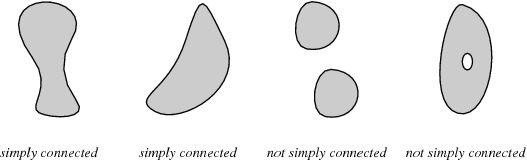
\includegraphics[width=400px]{img/simplyconnected.jpg}\end{center}

\proposition{Divergence Theorem}
Let $\textbf{F}:\real^3\to\real^3$ be a vector field and $V\subset\real^3$ be a simply connected domain with boundary $\partial V$.\\
The \textit{Divergence Theorem} states
$$\int_V\nabla\circ\textbf{F}dV=\int_{\partial V}\textbf{F}\circ d\textbf{S}=\int_{\partial V}\textbf{F}\circ\hat{\textbf{n}}dS$$
where $\hat{\textbf{n}}$ points out of $V$.\\
\textit{N.B.} - Proof is non-examinable.

\subsection{Green's Identities}

\remark{Not a Green's Identity}
Let $\textbf{F}=\nabla f$.\\
Then $\nabla\circ\textbf{F}=\nabla\circ\nabla f=\Delta f$.\\
By the divergence theorem
$$\implies\int_V\Delta fdV=\int_{\partial V}\hat{\textbf{n}}\nabla f dS$$

\proposition{Green's First Identity}
Let $f,g:\real^3\to\real$ be scalar fields $\textbf{F}:\real^3\to\real^3$.\\
Define $\textbf{F}=g\nabla f$.\\
Then \textit{Green's First Identity} states
$$\int_V(\nabla g\circ\nabla f)+(g\Delta f)dV=\int_{\partial V}g\hat{\textbf{n}}\circ\nabla fdS$$

\proposition{Green's Second Identity}
By subtracting the result of \textit{Green's First Identity} we have
$$\int_V(g\Delta f-f\Delta g)dV=\int_{\partial V}(g\hat{\textbf{n}}\circ\nabla f-f\hat{\textbf{n}}\circ\nabla g)dS$$


\setcounter{section}{-1}
\newpage\section{Reference}

\subsection{Notation}

\notation{Basis vectors}
\textit{Basis vectors} are donated by having a hat,$\hat{}$, over them.\\
\textit{Example} The basis vectors of $\real^3$ in Cartesian co-ordinates are
\[\begin{array}{rcccl}
\hat{\textbf{x}} &=& (1,0,0) &\equiv& \hat{\textbf{e}}_1\\
\hat{\textbf{y}} &=& (0,1,0) &\equiv& \hat{\textbf{e}}_2\\
\hat{\textbf{z}} &=& (0,0,1) &\equiv& \hat{\textbf{e}}_3
\end{array}\]

\notation{Boundary}
For a region $A\subset\real^n$ the \textit{boundary} of $A$ is denoted as
$$\partial A$$

\notation{Closed Loop Integral}
Let $C$ be a \textit{closed curve}.\\
An integral along $C$ can be denoted as
$$\int_C\nabla f\circ d\textbf{r}\equiv\oint_C\nabla f\circ d\textbf{r}$$

\notation{Curl}
The \textit{Curl} of a vector field $\textbf{v}:\real^3\to\real^3$ is denoted as
$$\nabla\times\textbf{v}$$

\notation{Direction}
Let $\textbf{v}\in\real^n$. The direction in $\textbf{v}$ is defined as
$$\textbf{\^v}=\dfrac{\textbf{v}}{|\textbf{v}|}$$

\notation{Directional Derivative}
The \textit{Directional Derivative} of the map $\textbf{F}:\real^m\to\real^n,\ m,n\in\nats$ at the point $\textbf{x}_0\in\real^m$ in the direction $\textbf{\^v}\in\real^m$ is denoted by
$$D_\textbf{\^v}\textbf{F}(\textbf{x}_0)$$

\notation{Divergence}
The \textit{Divergence} of a vector field $\textbf{v}:\real^3\to\real^3$ is denoted as
$$\nabla\circ\textbf{v}$$

\notation{Einstein Summation Convention}
The \textit{Einstein Summation Convention} is used to simplify summation formulae.\\
When indices are repeated it can be assumed that a summation is being used, thus the $\sum$ notation can be dropped.
$$\sum_{i=1}^nx_iy_i\implies x_iy_i$$
\textbf{But}, \textit{Greek} characters are used as indices when we don't want to imply summation.\\

\notation{Gradient}
The \textit{Gradient} of a scalar field $f:\real^3\to\real$ is denoted as
$$\nabla f$$

\notation{Isolating Vector Components}
Let $\textbf{v}\in\real^n$ for $n\in\nats$ and $i\in[1,n]$.\\
To isolate the $i^{th}$ component of the vector $\textbf{v}$ we use
$$[\textbf{v}]_i$$

\notation{Jacobian Determinant}
The \textit{Jacobian determinant} of the vector map $\textbf{F}$ is denoted
$$J_\textbf{F}$$

\notation{Kronecker Delta}
The \textit{Kronecker Delta} function of two variables which returns $1$ if they are the same, and $0$ otherwise.
$$\delta_{ij} = \begin{cases} 1\ \mathrm{if}\ i=j \\ 0\ \mathrm{otherwise}\end{cases}$$

\notation{Laplacian}
The \textit{Laplacian} of a scalar field $f:\real^3\to\real$ is denoted as
$$\Delta f$$
\textit{N.B.} - Occasionally it is denoted as $\nabla^2f$.\\

\notation{Levi-Civita Tensor}
 The \textit{Levi-Civita Tensor} describes the antisymmetric nature of vectors.\\
It is denoted in the form
$$\mathcal{E}_{ijk}\quad i,j,k\in\nats$$
It is defined by the following rules
\begin{enumerate}[label=\roman*)]
  \item $\mathcal{E}_{123}=1$.
  \item $\mathcal{E}_{ijk}=0$ if any suffices are repeated.
  \item Reversing any suffices negates the value of $\mathcal{E}_{ijk}$.
\end{enumerate}
\textit{N.B.} - This is occasionally know as \textit{antisymmetric symbol}.\\

\notation{Line Integral of Scalar Field}
The \textit{Line Integral} of a scalar field $f:\real^3\to\real$ along a curve $C$ is denoted
$$\int_Cf(\textbf{r})ds$$
where $ds=|d\textbf{r}|$.\\

\notation{Line Integral of Vector Field}
the \textit{Line Integral} of a vector field $\textbf{F}:\real^3\to\real^3$ along a curve $C$ is denoted as.
$$\int_C\textbf{F}(\textbf{r})\circ d\textbf{r}$$
\textit{N.B.} - $\circ$ is dot product here.\\

\notation{Position Vector, $\real^3$}
The general \textit{position vector} in $\real^3$ is often denoted by
$$\textbf{r}:=(x,y,z)$$

\notation{Vector Notation}
$\textbf{x} \in \real^m$ for $m \in \nats$ is used to denoted the vector $\begin{pmatrix} x_1 \\ \vdots \\ x_m \end{pmatrix}, x_i \in \real\ \forall\ i = \{1, \dots, m\}$.\\

\notation{Volume Integral of a Scalar Field}
Let $f(\textbf{r})$ be a scalar field.\\
The \textit{volume integral} of $f(\textbf{r})$ over $V\subset\real^3$ is denoted
$$\int_Vf(\textbf{r})dV\equiv\iiint_Vf(x,y,z)dxdydz$$

\subsection{Definitions}

\definition{Anti-Symmetric}
An operation is \textit{anti-symmetric} if reversing the order of its variables does not change the magnitude of the result, \textit{but} does swap the sign.\\
\textit{Example} - Cross-product.\\

\definition{Associative}
An operation is \textit{associative} if changing the order of its variables does not alter the outcome.\\
\textit{Example} - Addition.\\

\definition{Cross Product}
Let $\textbf{u}, \textbf{v} \in\real^3$ st $\textbf{u} = (u_1, u_2, u_3)\ \&\ \textbf{v}=(v_1, v_2, v_3)$.\\
The \textit{Cross product} of \textbf{u} \& \textbf{v} is defined
\[\begin{array}{rcl}
\textbf{u}\times\textbf{v}&:=&\begin{vmatrix}\hat{\textbf{e}}_1 & \hat{\textbf{e}}_2 & \hat{\textbf{e}}_3 \\ u_1 & u_2 & u_3 \\ v_1 & v_2 & v_3 \end{vmatrix}\\
&=&\hat{\textbf{e}}_1\begin{vmatrix} u_2 & u_3 \\ v_2 & v_3\end{vmatrix} - \hat{\textbf{e}}_2\begin{vmatrix} u_1 & u_3 \\ v_1 & v_3\end{vmatrix} + \hat{\textbf{e}}_3\begin{vmatrix} u_1 & u_2 \\ v_1 & v_2\end{vmatrix}\end{array}\]

\definition{Direction}
A \textit{Direction} is a vector of unit length
$$|\textbf{v}|=1$$

\definition{Dot Product}
Let $\textbf{u}, \textbf{v} \in\real^n$ st $\textbf{u} = (u_1, \dots, u_n)\ \&\ \textbf{v}=(v_1, \dots, v_n)$.\\
The \textit{Dot Product} of \textbf{u} \& \textbf{v} is defined
$$\textbf{u}\dotprod\textbf{v}:=u_iv_i=\sum_{i=1}^nu_iv_i$$

\definition{Hessian Matrix}
Let $f : \real^n \to \real$ be a scalar function.\\
The \textit{Hessian Matrix} is the square matrix representation of the second-order partial derivatives of $f$.
$$\textbf{H}=\begin{pmatrix}
\frac{\partial^2 f}{\partial x_1^2} & \frac{\partial^2 f}{\partial x_1 \partial x_2} & \dots & \frac{\partial^2 f}{\partial x_1 \partial x_n}\\
\frac{\partial^2 f}{\partial x_2 \partial x_1} & \frac{\partial^2 f}{\partial^2 x_2} & \dots & \frac{\partial^2 f}{\partial x_2 \partial x_n}\\
\vdots & \vdots & \ddots & \vdots\\
\frac{\partial^2 f}{\partial x_n \partial x_1} & \frac{\partial^2 f}{\partial x_n \partial x_2} & \dots & \frac{\partial^2 f}{\partial x_n^2}
\end{pmatrix}$$

\definition{Hyperbolic Trigonometric Functions}
\[\begin{array}{lll}
\sinh x=\dfrac{e^x-e^{-x}}{2}&\cosh x=\dfrac{e^x+e^{-x}}{2}&\tanh x=\dfrac{\sinh x}{\cosh x}\\
\cosech x=\dfrac{1}{\sinh x}&\sech x=\dfrac{1}{\cosh x}&\coth x=\dfrac{1}{\tanh x}
\end{array}\]

\definition{Level Curves/Surface}
\textit{Level curves/surfaces} are lines where $f(x,y)=c$ for some constant $c\in\real$.\\
\textit{N.B.} - Consider contour lines on an OS map.\\

\definition{Multi-Linear}
A multi-variable function is \textit{multi-linear} if it can be separated into multiple functions, each taking one variable, without altering the outcome.\\
\textit{i.e.} $f(\lambda x_1 + \mu x_2, y) = \lambda f(x_1, y)+\mu f(x_2, y)$.\\

\definition{Norm}
Let $\textbf{v}\in\real^n$ for $n\in\nats$.\\
The \textit{Norm} of $\textbf{v}$ is the strictly positive length of a $\textbf{v}$. $$|\textbf{v}| = \sqrt{\textbf{v} \dotprod \textbf{v}} = \sqrt{\sum_{i=1}^n v_i^2}$$

\definition{Orthogonal Matrix}
A matrix, $A\in M(\real)$ is \textit{orthogonal} if
$$A^TA=I\implies A^T=A^{-1}$$

\subsection{Theorems}

\theorem{Chain Rule}
\[\begin{array}{rcl}
[f(g(x))]' &=& f'(g(x)).g'(x)\\
(\textbf{F}\circ\textbf{G})'&=&(\textbf{F}'\circ\textbf{G})\textbf{G}'\\
\dfrac{dy}{dx} &=& \dfrac{dy}{dt}\dfrac{dt}{dx}
\end{array}\]

\stepcounter{theorem}\textbf{Theorem \arabic{section}.\arabic{theorem} - }{Common Curvilinear Co-Ordinate Systems}
\[\begin{array}{rrcccl}
Cylindrical&(x,y,z) &=& \textbf{r}(r,\theta,z) &=& (r\cos\theta,r\sin\theta,z)\\
Polar&(x,y) &=& \textbf{r}(r,\theta) &=& (r\cos\theta,r\sin\theta)\\
Spherical&(x,y,z) &=& \textbf{r}(r,\phi,\theta) &=& (r\sin\phi\cos\theta,r\sin\phi\theta,r\cos\phi)
\end{array}\]

\theorem{Derivative of Exponent}
$$[e^{f(x)}]'=f(x)'e^{f(x)}$$

\theorem{Derivative of Logarithms}
$$(\log_bf)'=\frac{f'}{\ln(b).f'}\quad(\ln f)'=\frac{f'}{f}$$

\theorem{Derivative of Hyperbolic Trigonometric Functions - Hyperbolic}
\[\begin{array}{lcl|lcl}
\frac{d}{dx}\sinh x&=&\cosh x&
\frac{d}{dx}\cosech x&=&-\cosech x\coth x\\
\frac{d}{dx}\cosh x&=&\sinh x&
\frac{d}{dx}\sech x&=&-\sech x\tanh x\\
\frac{d}{dx}\tanh x&=&\sech^2 x&
\frac{d}{dx}\coth x&=&-\cosech^2x
\end{array}\]

\theorem{Derivative of  Functions - Inverse}
\[\begin{array}{lcl|lcl}
\frac{d}{dx}\sin^{-1}x&=&\dfrac{1}{\sqrt{1-x^2}}&
\frac{d}{dx}\cosec^{-1}x&=&\dfrac{-1}{|x|\sqrt{x^2-1}}\\
\frac{d}{dx}\cos^{-1}x&=&\dfrac{-1}{\sqrt{1-x^2}}&
\frac{d}{dx}\sec^{-1}x&=&\dfrac{1}{|x|\sqrt{x^2-1}}\\
\frac{d}{dx}\tan^{-1}x&=&\dfrac{1}{1+x^2}&
\frac{d}{dx}\cot^{-1}x&=&\dfrac{-1}{1+x^2}
\end{array}\]

\theorem{Derivative of Trigonometric Functions - Standard}
\[\begin{array}{lcl|lcl}
\frac{d}{dx}\sin x&=&\cos x&
\frac{d}{dx}\cosec x&=&-\cosec x\cot x\\
\frac{d}{dx}\cos x&=&-\sin x&
\frac{d}{dx}\sec x&=&\tan x\sec x\\
\frac{d}{dx}\tan x&=&\sec^2x&
\frac{d}{dx}\cot x&=&-\cosec^2x
\end{array}\]

\theorem{Euler's Formula}
$$e^{ix}=\cos x+i\sin x$$

\theorem{Integration by Parts}
$$\int_a^budv=[uv]_a^b-\int_a^bvdu\Longleftrightarrow\int_a^budv+vdu=\int_a^bu\frac{dv}{dx}dx+v\frac{du}{dx}dx=\int_a^b\frac{d}{dx}(uv)dx=[uv]_b^a$$

\theorem{Product Rule}
$$(f.g)'=fg'+f'g$$

\theorem{Quotient Rule}
$$\left(\frac{f}{g}\right)'=\frac{f'g-g'f}{g^2}$$

\theorem{Trigonometric Identities - Hyperbolic}
\[\begin{array}{rcl|rcl}
\cosh^2\theta-\sinh^2\theta&=&1&
\tanh^2\theta+\sech^2\theta&=&1\\
\coth^2\theta-\cosech^2\theta&=&1\\
\sinh(\theta\pm\phi)&=&\sinh\theta\cosh\phi\pm\cosh\theta\sinh\phi&
\sinh(2\theta)&=&2\sinh\theta\cosh\theta\\
\cosh(\theta\pm\phi)&=&\cosh\theta\cosh\phi\pm\sinh\theta\sinh\phi&
\cosh(2\theta)&=&\cosh^2\theta+\sinh^2\theta\\
\tanh(\theta\pm\phi)&=&\dfrac{\tanh\theta\pm\tanh\phi}{1\pm\tanh\theta\tanh\phi}&\\
\sinh^2\theta&=&\dfrac{\cosh2\theta+1}{2}&
\cosh^2\theta&=&\dfrac{\cosh2\theta-1}{2}
\end{array}\]

\theorem{Trigonometric Identities - Standard}
\[\begin{array}{rcl|rcl}
\sin^2\theta+\cos^2\theta&=&1\\
\sin(\theta\pm\phi)&=&\sin\theta\cos\phi\pm\cos\theta\sin\phi&
\sin(2\theta)&=&2\sin\theta\cos\theta\\
\cos(\theta\pm\phi)&=&\cos\theta\cos\phi\mp\sin\theta\sin\phi&
\cos(2\theta)&=&\cos^2\theta-\sin^2\theta\\
\tan(\theta\pm\phi)&=&\dfrac{\tan\theta\pm\tan\phi}{1\mp\tan\theta\tan\phi}&
\tan(2\theta)&=&\dfrac{2\tan\theta}{1-\tan^2\theta}\\
\sin^2\theta&=&\dfrac{1-\cos2\theta}{2}&
\cos^2\theta&=&\dfrac{1+\cos2\theta}{2}\\
2\cos\theta\cos\phi&=&\cos(\theta-\phi)+\cos(\theta+\phi)&
2\sin\theta\sin\phi&=&\cos(\theta-\phi)-\cos(\theta+\phi)\\
2\sin\theta\cos\phi&=&\sin(\theta+\phi)+\sin(\theta-\phi)&
2\cos\theta\sin\phi&=&\sin(\theta+\phi)-\sin(\theta-\phi)\\
\sin(-x)&=&-\sin(x)&
\end{array}\]
\end{document}
